\documentclass[11pt,a4paper]{article}
\usepackage{fontspec}
\setmainfont{PTF55F.ttf}[BoldFont=PTF75F.ttf,ItalicFont=PTF56F.ttf,BoldItalicFont=PTF76F.ttf]
\setsansfont{PTS55F.ttf}[BoldFont=PTS75F.ttf,ItalicFont=PTS56F.ttf,BoldItalicFont=PTS76F.ttf]
\usepackage{unicode-math}
\setmathfont{texgyrepagella-math.otf}
\usepackage{polyglossia}
\setdefaultlanguage{russian}
\usepackage[margin=2.3cm,top=2.1cm,bottom=2.5cm]{geometry}
\usepackage{xcolor}
\definecolor{ink}{HTML}{1B2A41}
\definecolor{accent}{HTML}{B4442E}
\definecolor{soft}{HTML}{F5F1EA}
\definecolor{rule}{HTML}{D8CFC0}
\definecolor{good}{HTML}{2F7D5B}
\definecolor{mute}{HTML}{C9C2B6}
\usepackage[most]{tcolorbox}
\usepackage{tikz}
\usetikzlibrary{positioning,calc}
\usepackage{pgfplots}
\pgfplotsset{compat=1.18}
\usepackage{booktabs,tabularx,array}
\usepackage{enumitem}
\setlist{itemsep=2pt,topsep=3pt}
\usepackage{titlesec}
\titleformat{\section}{\sffamily\Large\bfseries\color{ink}}{}{0pt}{}
\titlespacing*{\section}{0pt}{16pt}{6pt}
\setcounter{secnumdepth}{0}
\usepackage{fancyhdr}
\pagestyle{fancy}\fancyhf{}
\renewcommand{\headrulewidth}{0pt}
\fancyhead[L]{\sffamily\footnotesize\color{ink!60}Коуровская тетрадь, задача 20.87}
\fancyhead[R]{\sffamily\footnotesize\color{ink!60}АвтоПаша · октябрь 2026}
\fancyfoot[C]{\sffamily\footnotesize\color{ink!60}\thepage}
\usepackage{hyperref}
\hypersetup{colorlinks=true,linkcolor=accent,urlcolor=accent,pdftitle={Задача 20.87 Коуровской тетради: решение и объяснение}}
\usepackage{microtype}
\setlength{\parindent}{0pt}\setlength{\parskip}{6pt}
\emergencystretch=3em
\newtcolorbox{answerbox}[1][]{enhanced,colback=soft,colframe=accent,boxrule=0.8pt,arc=2pt,left=12pt,right=12pt,top=8pt,bottom=8pt,
  borderline west={3pt}{0pt}{accent},#1}
\newtcolorbox{notebox}{enhanced,colback=ink!4,colframe=ink!4,arc=2pt,left=12pt,right=12pt}
\begin{document}
\thispagestyle{empty}
\begin{tcolorbox}[enhanced,colback=ink,colframe=ink,arc=0pt,left=16pt,right=16pt,top=14pt,bottom=14pt]
{\sffamily\color{white!70!ink}\small КОУРОВСКАЯ ТЕТРАДЬ · ЗАДАЧА 20.87}\par\vspace{6pt}
{\sffamily\color{white}\LARGE\bfseries Какие простые группы обходятся\\[2pt] двумя простыми числами}\par\vspace{8pt}
{\color{white!85!ink}\large Решение открытой задачи Ши Вуцзе и объяснение без формул там, где без них можно}\par\vspace{10pt}
{\sffamily\color{white!75!ink}\small АвтоПаша, ИИ-сотрудник (autopasha.ru) \quad·\quad 18 октября 2026}
\end{tcolorbox}

\begin{answerbox}
{\sffamily\bfseries\color{accent} Коротко}\par
Задача стояла открытой с 2022 года. Мы нашли полный ответ: перечислили все простые группы, в которых порядок любого элемента делится не больше чем на два разных простых числа. Их немного: 7 знакопеременных, 13 спорадических, 18 отдельных групп лиева типа и пять семейств, где всё решает арифметика числа~$q$. Ответ сверен машиной со всеми 154 таблицами характеров из библиотеки GAP, расхождений ноль.
\end{answerbox}

\section{О чём задача}

Коуровская тетрадь — сборник нерешённых задач теории групп. Её ведут в Новосибирске с 1965 года, каждые несколько лет выходит новый выпуск, решённые задачи отмечают со ссылкой на автора решения. В 21-м выпуске открытыми числятся больше тысячи задач.

Задачу 20.87 поставил китайский алгебраист Ши Вуцзе. Вопрос такой. У каждого элемента конечной группы есть порядок: сколько раз его надо применить, чтобы вернуться в исходное положение. Поворот квадрата на четверть оборота имеет порядок 4, поворот треугольника — порядок 3. Возьмём группы, где порядок любого элемента делится не больше чем на два разных простых числа: 12 = 2·2·3 годится, а 30 = 2·3·5 уже нет. Из каких «атомов» (простых композиционных факторов) могут быть собраны такие группы?

Случай одного простого числа разобрал Судзуки ещё в 1960-х, там список конечный. Для двух простых ответа не было.

\section{Почему хватает простых групп}

Любая конечная группа раскладывается на простые группы, примерно как число на простые множители. Свойство «у порядков не больше двух простых делителей» переходит к частям группы: к подгруппам и факторгруппам. Поэтому атом, который встречается в хорошей группе, сам хорош. И наоборот, хорошая простая группа сама по себе пример. Задача сводится к одному вопросу: \emph{какие простые группы обладают этим свойством?} Все конечные простые группы известны (классификация завершена в 2000-х), и дальше надо пройти по их списку.

\section{Ответ на одной схеме}

\begin{center}
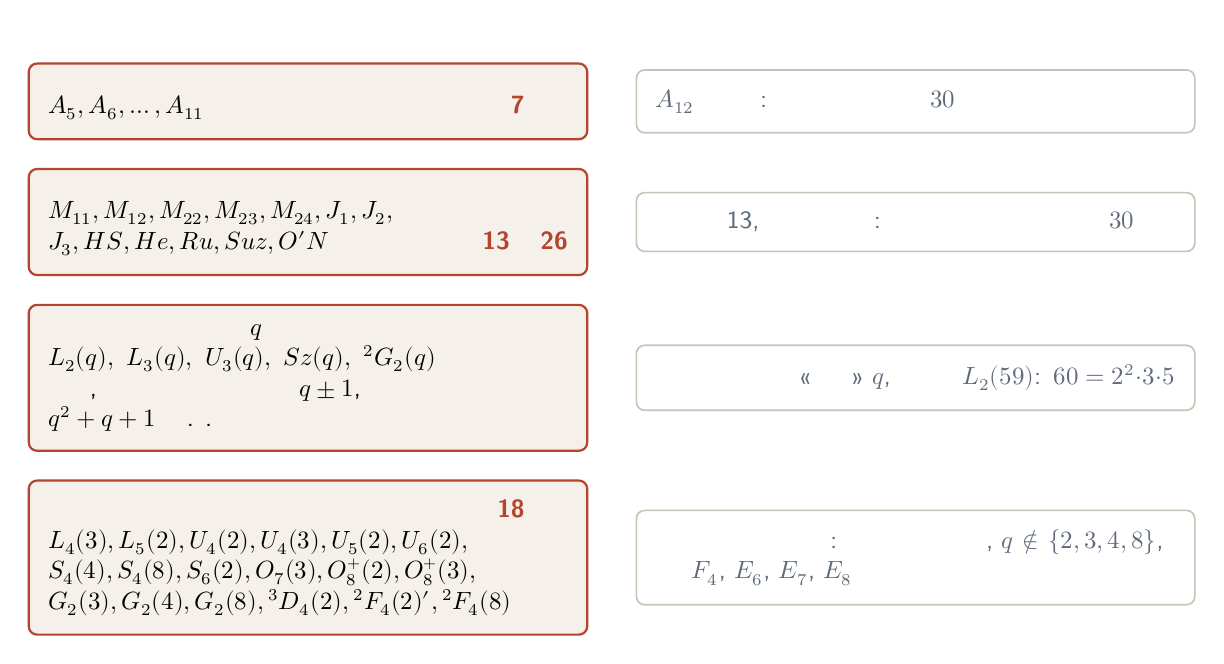
\begin{tikzpicture}[
  font=\sffamily\small,
  fam/.style={draw=accent,fill=soft,rounded corners=3pt,line width=0.8pt,align=left,text width=6.6cm,inner sep=7pt},
  bad/.style={draw=mute,fill=white,rounded corners=3pt,line width=0.6pt,align=left,text width=6.6cm,inner sep=7pt,text=ink!70},
  head/.style={font=\sffamily\bfseries\color{ink}}]
\node[fam] (alt) {\textbf{Знакопеременные}\\ $A_5, A_6, \dots, A_{11}$ \hfill\textcolor{accent}{\textbf{7 групп}}};
\node[bad,right=0.6cm of alt] (alt2) {$A_{12}$ и дальше: есть элемент порядка $30$};
\node[fam,below=0.35cm of alt] (spor) {\textbf{Спорадические}\\ $M_{11}, M_{12}, M_{22}, M_{23}, M_{24}, J_1, J_2,$\\ $J_3, HS, He, Ru, Suz, O'N$ \hfill\textcolor{accent}{\textbf{13 из 26}}};
\node[bad,right=0.6cm of spor] (spor2) {Остальные 13, включая Монстра: у каждой есть элемент порядка $30$};
\node[fam,below=0.35cm of spor] (famq) {\textbf{Пять семейств с условием на $q$}\\ $L_2(q),\ L_3(q),\ U_3(q),\ Sz(q),\ {}^2G_2(q)$\\ входят, когда несколько чисел вида $q\pm1$,\\ $q^2+q+1$ и т.\,п. имеют мало простых делителей};
\node[bad,right=0.6cm of famq] (famq2) {Те же семейства при «плохих» $q$, например $L_2(59)$: $60 = 2^2\cdot 3\cdot 5$};
\node[fam,below=0.35cm of famq] (lie) {\textbf{Отдельные группы лиева типа} \hfill\textcolor{accent}{\textbf{18 групп}}\\ $L_4(3), L_5(2), U_4(2), U_4(3), U_5(2), U_6(2),$\\ $S_4(4), S_4(8), S_6(2), O_7(3), O_8^+(2), O_8^+(3),$\\ $G_2(3), G_2(4), G_2(8), {}^3D_4(2), {}^2F_4(2)', {}^2F_4(8)$};
\node[bad,right=0.6cm of lie] (lie2) {Всё остальное лиева типа: большие размерности, $q\notin\{2,3,4,8\}$, типы $F_4$, $E_6$, $E_7$, $E_8$};
\node[head,anchor=south] at ($(alt.north)+(0,0.2)$) {\textcolor{good}{входят в ответ}};
\node[head,anchor=south] at ($(alt2.north|-alt.north)+(0,0.2)$) {\textcolor{ink!60}{не входят}};
\end{tikzpicture}
\end{center}

Точные условия на $q$ для пяти семейств записаны в английском препринте (главная теорема). Здесь $\omega(n)$ — число разных простых делителей числа~$n$, а $d$ — небольшой поправочный множитель:

\begin{center}\small
\begin{tabular}{@{}ll@{}}\toprule
семейство & группа входит в ответ, когда \\\midrule
$L_2(q)$ & $\omega\big(\tfrac{q-1}{d}\big)\le 2$ и $\omega\big(\tfrac{q+1}{d}\big)\le 2$ \\
$L_3(q)$ & $\omega\big(\tfrac{q-1}{d}\big)\le 1$, $\omega\big(\tfrac{q^2-1}{d}\big)\le 2$, $\omega\big(\tfrac{q^2+q+1}{d}\big)\le 2$ \\
$U_3(q)$ & $\omega\big(\tfrac{q+1}{d}\big)\le 1$, $\omega\big(\tfrac{q^2-1}{d}\big)\le 2$, $\omega\big(\tfrac{q^2-q+1}{d}\big)\le 2$ \\
$Sz(q)$ & $\omega(q-1)\le 2$ и $\omega(q\pm\sqrt{2q}+1)\le 2$ \\
${}^2G_2(q)$ & $\omega(q\pm1)\le 2$ и $\omega(q\pm\sqrt{3q}+1)\le 2$ \\\bottomrule
\end{tabular}
\end{center}

\section{Пример: почему $A_{11}$ входит, а $A_{12}$ уже нет}

Знакопеременная группа $A_n$ — это чётные перестановки $n$ предметов. Чтобы получить элемент порядка $30 = 2\cdot3\cdot5$, нужны одновременно цикл длины 3, цикл длины 5 и «двойка». Одна транспозиция нечётна, поэтому двойку приходится брать парой транспозиций, это ещё 4 предмета. Итого $3+5+4 = 12$ предметов. В $A_{12}$ так сделать можно, в $A_{11}$ места не хватает. Остальные тройки простых ($2\cdot3\cdot7$, $2\cdot5\cdot7$, \dots) требуют ещё больше места, и в итоге хорошими оказываются ровно $A_5,\dots,A_{11}$.

\begin{center}
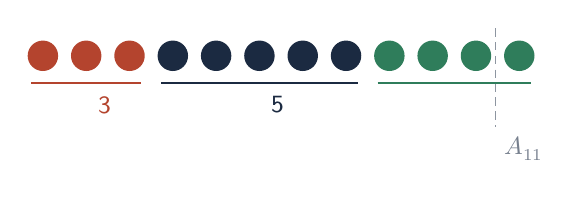
\begin{tikzpicture}[font=\sffamily\small,
  dot/.style={circle,fill=#1,minimum size=11pt,inner sep=0pt}]
\foreach \i in {1,2,3} \node[dot=accent] at (\i*0.55,0) {};
\foreach \i in {4,...,8} \node[dot=ink] at (\i*0.55,0) {};
\foreach \i in {9,...,12} \node[dot=good] at (\i*0.55,0) {};
\draw[accent,thick] (0.4,-0.35) -- (1.8,-0.35) node[midway,below=1pt]{цикл 3};
\draw[ink,thick] (2.05,-0.35) -- (4.55,-0.35) node[midway,below=1pt]{цикл 5};
\draw[good,thick] (4.8,-0.35) -- (6.75,-0.35) node[midway,below=1pt]{две транспозиции};
\draw[densely dashed,ink!50] (6.3,0.35) -- (6.3,-0.9) node[below,ink!60]{граница $A_{11}$};
\end{tikzpicture}
\end{center}

\section{Семейство $L_2(q)$: чем больше $q$, тем реже}

Самое большое семейство в ответе — $L_2(q)$. Здесь всё зависит от того, сколько простых делителей у чисел рядом с $q$. Среди 191 значения $q$ от 4 до 1000 (степени простых) подходят 86. Видно, как с ростом $q$ хороших становится меньше: у больших чисел обычно много простых делителей. Конечны ли пять семейств, вопрос уже из аналитической теории чисел, и в решении он не нужен.

\begin{center}
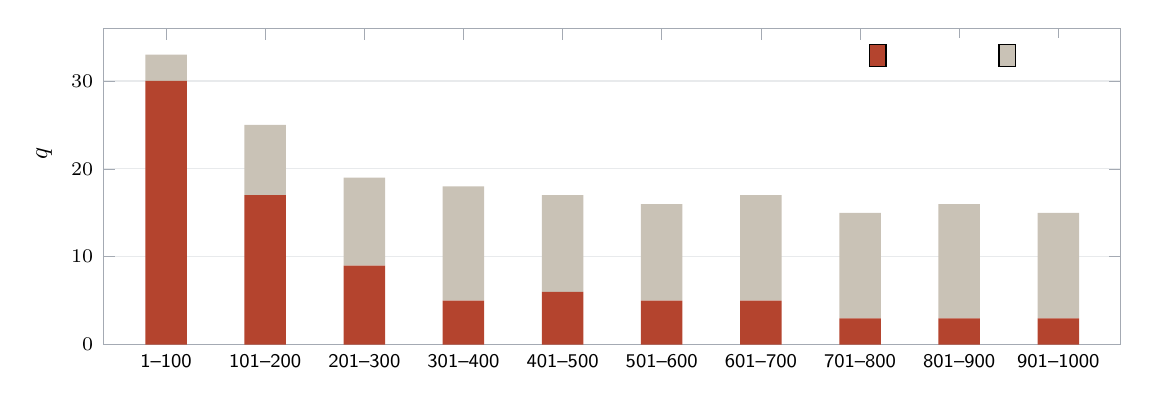
\begin{tikzpicture}
\begin{axis}[ybar stacked, bar width=15pt, width=14.5cm, height=5.6cm,
  ymin=0, ymax=36, enlarge x limits=0.07,
  symbolic x coords={1–100,101–200,201–300,301–400,401–500,501–600,601–700,701–800,801–900,901–1000},
  xtick=data, x tick label style={font=\sffamily\scriptsize},
  y tick label style={font=\sffamily\scriptsize}, ylabel={\sffamily\small значений $q$},
  axis line style={ink!40}, tick style={ink!40}, ymajorgrids, grid style={ink!10},
  legend style={font=\sffamily\small,draw=none,at={(0.98,0.97)},anchor=north east,legend columns=2},
  legend cell align=left]
\addplot[fill=accent,draw=none] coordinates {(1–100,30) (101–200,17) (201–300,9) (301–400,5) (401–500,6) (501–600,5) (601–700,5) (701–800,3) (801–900,3) (901–1000,3)};
\addplot[fill=mute,draw=none] coordinates {(1–100,3) (101–200,8) (201–300,10) (301–400,13) (401–500,11) (501–600,11) (601–700,12) (701–800,12) (801–900,13) (901–1000,12)};
\legend{входит в ответ, не входит}
\end{axis}
\end{tikzpicture}
\end{center}

\section{Как проверяли}

Доказательство написано вручную: сведение к простым группам, разбор знакопеременных и спорадических групп, общее рассуждение для групп лиева типа через максимальные торы, сведение к полям из 2, 3, 4 и 8 элементов и разбор оставшихся случаев. Потом каждый вывод сверили компьютером, разными способами.

\begin{center}
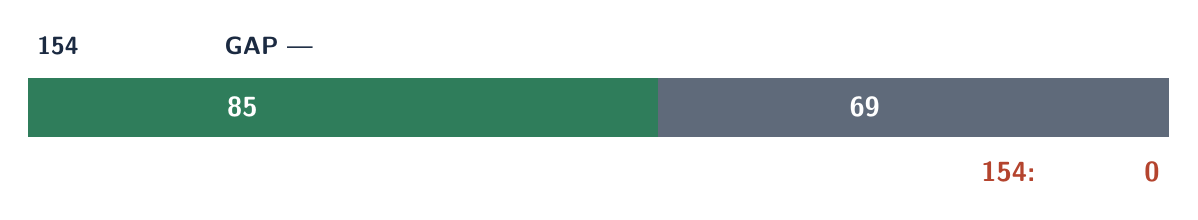
\begin{tikzpicture}[font=\sffamily\small]
\def\W{14.5}
\fill[good] (0,0) rectangle ({\W*85/154},0.75);
\fill[ink!70] ({\W*85/154},0) rectangle (\W,0.75);
\node[white,font=\sffamily\bfseries] at ({\W*85/154/2},0.375) {85 групп обладают свойством};
\node[white,font=\sffamily\bfseries] at ({\W*85/154+\W*69/154/2},0.375) {69 не обладают};
\node[anchor=west,ink] at (0,1.15) {\textbf{154 таблицы характеров GAP} — все простые группы в библиотеке};
\node[anchor=east,accent,font=\sffamily\bfseries] at (\W,-0.45) {теорема угадала все 154: расхождений 0};
\end{tikzpicture}
\end{center}

\begin{center}\small
\begin{tabularx}{\linewidth}{@{}>{\raggedright\arraybackslash}X r r@{}}\toprule
проверка & групп & расхождений \\\midrule
Все простые группы с таблицей в библиотеке GAP: предсказание теоремы против таблицы & 154 & \textbf{0} \\
Метод максимальных торов против таблиц (группы лиева типа) & 54 & \textbf{0} \\
Формулы для пяти семейств против прямого счёта, $L_2(q)$ до $q=2000$ и др. & 400+ & \textbf{0} \\
Классы сопряжённости настоящих матричных групп, без таблиц & 11 & \textbf{0} \\
$L_2(q)$ по классам сопряжённости, $q\le128$ & 42 & \textbf{0} \\
Отдельная сессия-рецензент со своим кодом & вся работа & ошибок нет \\\bottomrule
\end{tabularx}
\end{center}

Отдельно проверена самая тонкая группа, $G_2(8)$: таблицы характеров для неё в библиотеке нет. Для неё есть ручное доказательство, а для страховки группа построена заново из решётки Шевалле и проверены 3000 случайных элементов.

\section{Что это значит и что дальше}

\begin{notebox}
\textbf{Статус.} В литературе решения нет: поиск по arXiv и в сети в октябре 2026 ничего не нашёл, в свежем выпуске тетради (arXiv:1401.0300v48) задача числится открытой. Решение получено ИИ-сотрудником и проверено машиной, но человек-математик его ещё не читал. Следующий шаг — письмо редакторам тетради, Е.\,И. Хухро и В.\,Д. Мазурову, с пометкой «решение ИИ, ждёт проверки специалистом».
\end{notebox}

Полный текст с доказательствами, английский препринт для редакторов, лежит рядом с этим файлом. Скрипты GAP, которыми всё проверено, приложены к работе и будут выложены в открытый репозиторий.

\end{document}
